\section{Detailed properties of the three-mode chain}
\label{sec:short-chain}

The three-mode system is the smallest chain with an unforced interior degree
of freedom.  It is therefore a useful setting in which to ask two questions
that are difficult to isolate in long chains: whether the full stationary
density can be reconstructed in the reduced five-dimensional state space, and
which relaxation modes are actually visible in stationary trajectories.  We
treat these as separate inference problems.  In particular, a successful
trajectory fit is not taken as evidence for a stationary Fokker--Planck
solution unless it first passes an equilibrium known-answer test.

\subsection{Stationary state and the validation boundary}
\label{sec:short-chain-density}

We use the reduced state
\begin{equation}
 X=(I_1,I_2,I_3,\theta_1,\theta_3),
 \qquad \theta_r=2(\phi_r-\phi_2),\quad r\in\{1,3\},
\end{equation}
and the energy
\begin{equation}
 E(X)=\frac12 M^2-\frac14\sum_{j=1}^3 I_j^2
      +I_1I_2\cos\theta_1+I_2I_3\cos\theta_3,
 \qquad M=I_1+I_2+I_3.
\end{equation}
At equal bath temperatures, the exact invariant density with respect to
$dI_1dI_2dI_3d\theta_1d\theta_3$ is proportional to $\exp[-E(X)/T]$.
This Gibbs state provides a stronger validation target than agreement with
histograms alone, because it tests both the density and the stationary adjoint
equation.

The controlled trajectories were generated using double precision, fixed
timesteps, standard trigonometric functions, implicit-midpoint Hamiltonian
updates, Cartesian bath increments, and no positive-action projection.  For
each bath condition and timestep, complete trajectories---not individual
snapshots---were assigned to 32 training, 16 validation, and 16 blind-test
streams.  The minimum effective sample sizes on the fine-timestep test splits
were $1.16\times10^4$ out of equilibrium and $1.39\times10^4$ at equilibrium,
above the preregistered threshold of $5\times10^3$.

We tested a normalized conditional mixture in the logarithmic actions.  The
model combines a Gaussian mixture for $u_j=\log I_j$ with conditional periodic
von Mises factors for $(\theta_1,\theta_3)$, and includes the Jacobian
$\rho(I,\theta)=p(u,\theta)/(I_1I_2I_3)$.  Before fitting, we froze six model
families ($K=8$ or $16$, two network widths, and two stationary-equation
penalties) and three seeds per family.  Selection was allowed only if all
three seeds reproduced the equilibrium Gibbs slope and satisfied pointwise
$L^\dagger\rho=0$ residual gates.

Figure~\ref{fig:short-chain-density-gates} shows the complete equilibrium
validation result.  Although several likelihood fits reproduce the Gibbs
log-density slope approximately, none solves the stationary equation at the
declared accuracy.  Across the 18 fits, the median of
$|L^\dagger\rho/\rho|$ is $1.13$--$2.62$ (gate $0.20$), and its 90th
percentile is $3.71$--$9.46$ (gate $1.00$).  The centered Gibbs log-density
RMSE is $0.302$--$0.595$.  Hence no architecture is admissible, even before
opening the equilibrium blind split.

\begin{figure}[t]
  \centering
  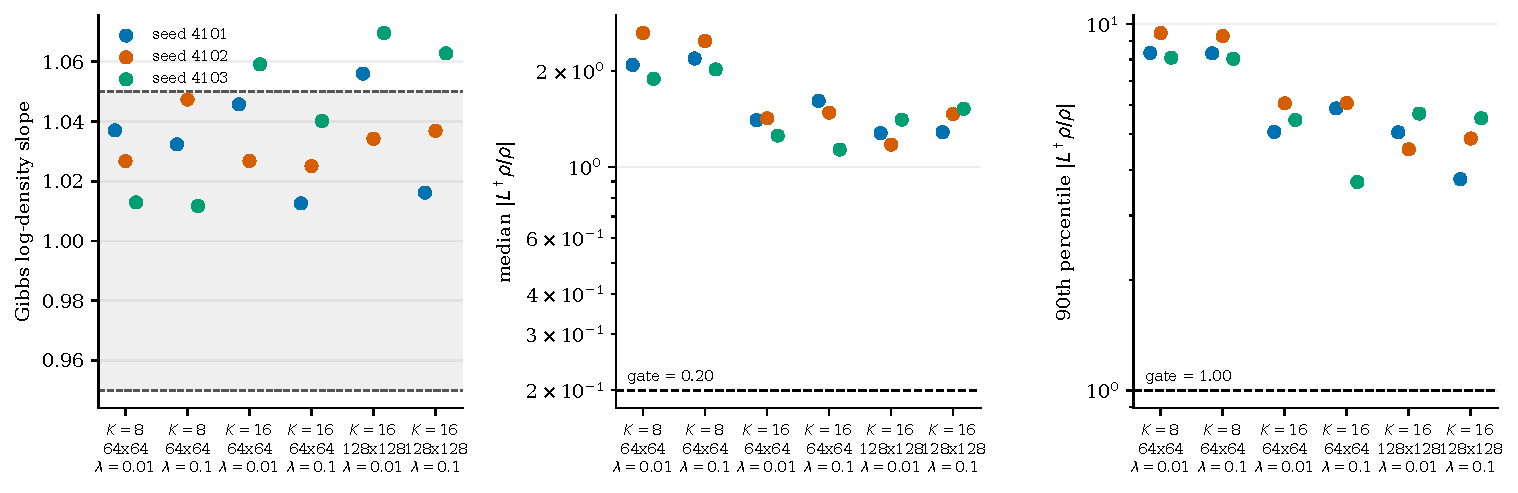
\includegraphics[width=\linewidth]{../figures/equilibrium_density_candidate_gates.pdf}
  \caption{Equilibrium known-answer calibration of the normalized stationary-
  density candidates.  Each symbol is one independent training seed.  The
  shaded region in the left panel is the validation slope gate; dashed lines
  in the residual panels are the preregistered pointwise Fokker--Planck gates.
  All candidates violate the residual gates.}
  \label{fig:short-chain-density-gates}
\end{figure}

This is a negative but decisive result: the tested neural family does not
support a numerical-solution claim for the five-dimensional stationary
Fokker--Planck equation.  In accordance with the frozen protocol, we did not
train the corresponding NESS density.  Consequently, density-derived claims
about low-probability stationary geometry are not used below.

\subsection{What is established about stabilization}
\label{sec:short-chain-stabilization}

The failure above concerns density reconstruction, not the existence of a
stationary trajectory ensemble.  Independent audits of the reduced generator
give maximum drift and covariance discrepancies of $2.3\times10^{-13}$ and
$2.9\times10^{-11}$, respectively, while the Gibbs adjoint residual is
$1.5\times10^{-14}$ in RMS on prespecified interior points.  Moreover, a
simultaneous equilibrium calibration of 18 regular weak identities yields a
family-wise threshold of $3.748$ standard errors, with no failures on the
equilibrium or driven held-out trajectories.  These tests support the use of
the controlled trajectories for stationary expectations and dynamical
correlations.

They do not, however, identify a quantitative high- versus low-energy
stabilization mechanism in the full state space.  Such an interpretation
would require either a stationary density that passes the Gibbs and adjoint
tests above, or a separate set of directly estimable conditional balance
relations with their own held-out controls.  We therefore leave the detailed
density geometry unresolved instead of inferring it from an unvalidated
neural solution.

\subsection{Held-out relaxation modes of the generator}
\label{sec:short-chain-modes}

The spectral analysis is independent of the density reconstruction.  We fit
extended dynamic mode decomposition (EDMD) operators on 32 trajectories,
selected dictionaries and regularization on 16 validation trajectories, and
froze the eigenvectors before a single evaluation on 16 test trajectories.
The dictionary includes raw endpoint-action differences and their prescribed
cross terms with the angular basis, so that it can represent the known
exchange-odd oscillation.  The slow real candidate is selected at lag
$\tau=0.5$, whereas the complex candidate is selected at $\tau=0.05$ to avoid
principal-log aliasing.

The selected slow real eigenvalues lie between $-0.91$ and $-0.95$ across bath
conditions and timesteps.  On the blind trajectories, their observable
autocorrelations yield rates $-0.884$ and $-0.909$ in the driven system, and
$-0.951$ and $-0.826$ at equilibrium, for timesteps $10^{-3}$ and
$2.5\times10^{-4}$, respectively.  As shown in
Fig.~\ref{fig:short-chain-heldout-modes}, the corresponding bootstrap intervals
overlap between timesteps and the held-out Koopman residuals do not grow by
more than the preregistered 25\% tolerance.

\begin{figure}[t]
  \centering
  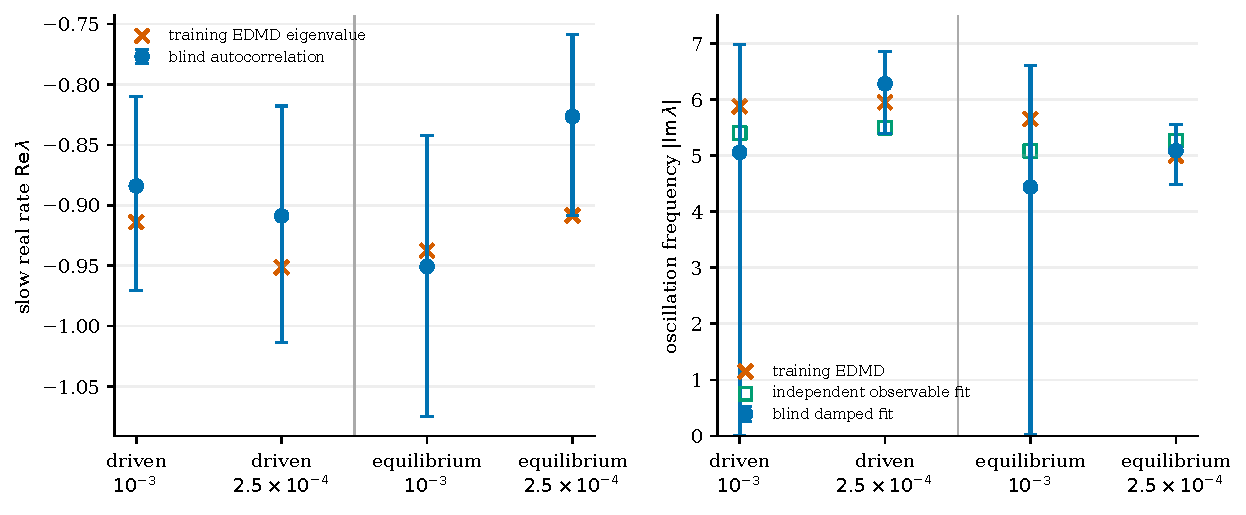
\includegraphics[width=\linewidth]{../figures/heldout_relaxation_modes.pdf}
  \caption{Held-out validation of the real and oscillatory EDMD modes.  Left:
  selected training eigenvalues and rates measured from the frozen
  eigenfunctions on blind trajectories.  Right: EDMD frequencies, independent
  observable-level fits, and blind damped-oscillation fits.  The coarse-step
  blind intervals are broad; the fine-step fits provide the informative
  frequency comparison.}
  \label{fig:short-chain-heldout-modes}
\end{figure}

The targeted complex mode is recovered as well.  At the fine timestep, the
blind frequencies are $6.281$ with 95\% interval $[5.388,6.862]$ in the driven
case and $5.088$ with interval $[4.487,5.558]$ at equilibrium.  These intervals
contain the independent observable-level estimates $5.500$ and $5.264$.
The coarse-timestep intervals exclude zero only narrowly and are much broader,
so we do not use them for a precision claim.

Finally, the slow eigenfunction has a reproducible observable content
(Fig.~\ref{fig:short-chain-mode-weights}).  Its absolute modal weight is
$0.47$--$0.50$ in $I_2$, $0.28$--$0.30$ in $I_1+I_3$, $0.20$--$0.22$ in the
cosine sum, and $0.106$--$0.124$ in $\cos\theta_3$.  This ordering explains why
different raw observables approach their asymptotic correlation rates with
different visibility, without requiring a different leading mode for each
observable.

\begin{figure}[t]
  \centering
  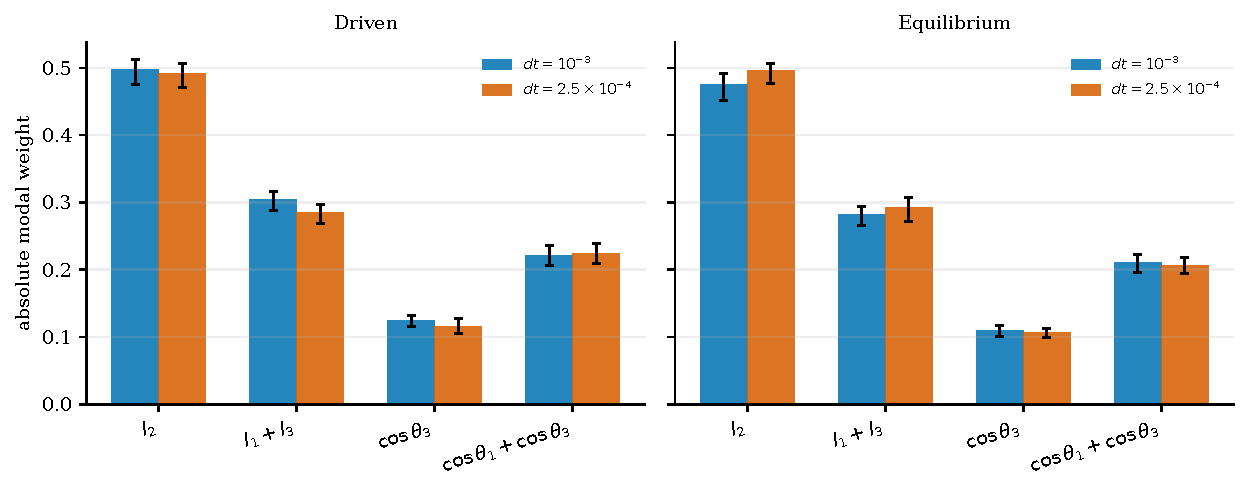
\includegraphics[width=\linewidth]{../figures/blind_slow_mode_weights.pdf}
  \caption{Absolute weights of four observables in the frozen slow real mode,
  evaluated on blind trajectories.  Error bars are 95\% whole-trajectory
  bootstrap intervals.  The ordering is stable across bath conditions and
  timesteps.}
  \label{fig:short-chain-mode-weights}
\end{figure}

The available evidence therefore resolves a held-out, EDMD-visible slow mode
and a faster damped oscillation.  It does not establish that the real mode is
the unique spectral gap of the full generator: the preregistered common-
autocorrelation-plateau gate still fails.  We retain this distinction in all
subsequent claims.
